% This is comment

\documentclass{article}

\usepackage[left=2.54cm, right=2.54cm, top=2.54cm, bottom=2.54cm]{geometry}
\usepackage{titlesec, amsmath, float}
\usepackage{epsfig}

\usepackage[round]{natbib}
\author{Tiffany\\MA DMF\\New Bedford, MA}
\date{}
\title{My first document}

% Section formatting
\titleformat{\section}{\Large\bfseries}{}{0pt}{}
\titleformat{\subsection}{\normalfont\bfseries\itshape}{}{0pt}{}
\titleformat{\subsubsection}{\normalfont\itshape}{}{0pt}{}

\begin{document}
\maketitle	

\tableofcontents

\listoffigures
\listoftables	
Objective 1 is complete! It's 20\% \$ \# It's 50$^\circ$. There some stuff in Table \ref{Table:df}.

some text, and a citation \citep{benoit2015generalized, maunder2004standardizing}.

\[ \hat{Y_i} = \beta_0 + \beta_1 + \epsilon_i  \]

\begin{eqnarray}
\eta = \sigma + X \\
\hat{Y_i} = \beta_0 + \beta_1 + \epsilon_i
\end{eqnarray}

\begin{equation}
\hat{Y_i} = \beta_0 + \beta_1 + \epsilon_i
\end{equation}



\section{Introduction}
 Some more text.
 
\section{Methods}
Plain text, wherever you want.
\subsection{Data}
My tog picture is in Figure \ref{Fig:tog}.

\begin{figure}[H]
	\centering
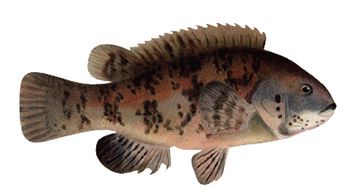
\includegraphics[scale=0.5]{tog.jpg}
\caption{A tog picture.}
\label{Fig:tog}
\end{figure}

\begin{itemize}
	\item item 1
	\item item 2
	\item item 3
\end{itemize}

\begin{enumerate}
	\item item 1
	\item item 2
	\item item 3
\end{enumerate}


\bibliographystyle{apalike}
\bibliography{References}


\begin{table}[ht]
	\centering
	\begin{tabular}{rr}
		\hline
		Year & Value \\ 
		\hline
		2000 & 6 \\ 
		2001 & 4 \\ 
		2002 & 5 \\ 
		2003 & 7 \\ 
		2004 & 2 \\ 
		2005 & 3 \\ 
		2006 & 6 \\ 
		2007 & 1 \\ 
		2008 & 6 \\ 
		2009 & 6 \\ 
		2010 & 6 \\ 
		2011 & 6 \\ 
		2012 & 3 \\ 
		2013 & 5 \\ 
		2014 & 4 \\ 
		2015 & 6 \\ 
		2016 & 6 \\ 
		\hline
		2017 & 6 \\ 
	\end{tabular}
	\caption{Printing data frame df using xtable.} 
	\label{Table:df}
\end{table}

	
\end{document}

% latex table generated in R 3.4.1 by xtable 1.8-2 package
% Thu Mar 01 10:56:23 2018

% latex table generated in R 3.4.1 by xtable 1.8-2 package
% Thu Mar 01 12:09:48 2018
\begin{table}[ht]
\centering
\begin{tabular}{rr}
  \hline
Year & Value \\ 
  \hline
2000 & 2 \\ 
  2001 & 8 \\ 
  2002 & 3 \\ 
  2003 & 3 \\ 
  2004 & 1 \\ 
  2005 & 4 \\ 
  2006 & 4 \\ 
  2007 & 4 \\ 
  2008 & 5 \\ 
  2009 & 6 \\ 
  2010 & 3 \\ 
  2011 & 2 \\ 
  2012 & 3 \\ 
  2013 & 5 \\ 
  2014 & 5 \\ 
  2015 & 4 \\ 
  2016 & 7 \\ 
   \hline
2017 & 6 \\ 
  \end{tabular}
\caption{Printing data frame df using xtable.} 
\label{Table:df}
\end{table}
